\section{Results}
First, we tested the model with the perception data. 
Our model was able to classify the 12-classes (12 stimuli listed in \autoref{tab:stimuli_information}) with a 28.7\% accuracy rate (chance = 8.3\%) at a significance level of p=0.001. 
Significance values were determined by using the cumulative binomial distribution to estimate the likelihood of observing a given classification rate by chance. 
\autoref{fig:model_W_confusion} is a confusion matrix which shows the classification results for each stimulus.
\begin{figure}[htb] 
  \begin{center}
    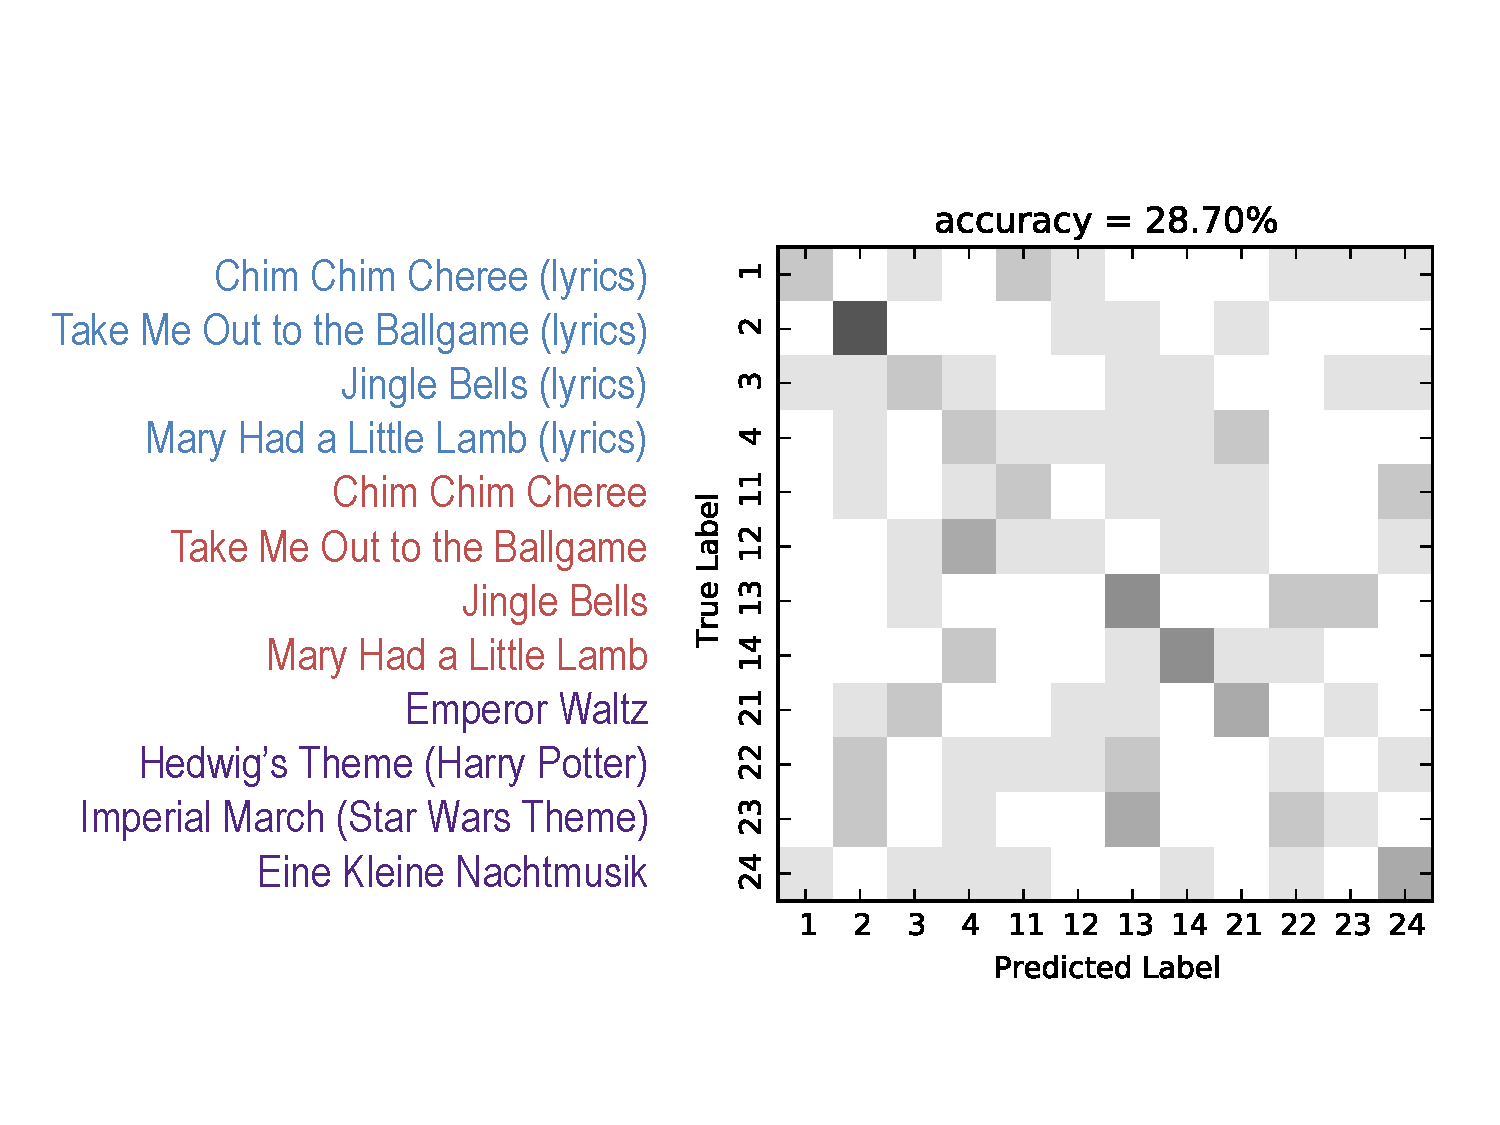
\includegraphics[width=.75\textwidth,keepaspectratio=true]{Figures/model_W_confusion}
   \\\vspace{-0.8em}
    \caption{12-class confusion matrix for perception data. Colour indicates the number of times each selection was made with darker colours indicating more selections.}
    \label{fig:model_W_confusion}
  \end{center}
%  \vspace{-1em}
\end{figure}
From the confusion matrix we can see that some stimuli are more accurately classified than others. 
Stimulus 2 is the most accurately classified. 
Stimuli 13 and 14 are also classified with some accuracy, and some confusion with their lyric counterparts (stimuli 3 and 4) can be seen.
Confusion between lyric and non-lyric pairs can also be seen with stimulus 1 being classified as stimulus 11.

To further investigate which pairs of stimuli our classifier can distinguish best we put all combinations of paired stimuli through our classifier.
This resulted in the series of binary confusion matrices in \autoref{fig:model_W_binary_confusion} that show us that some pairs of stimuli are more easily differentiated from each other than others. 
\begin{figure}[htb] 
  \begin{center}
    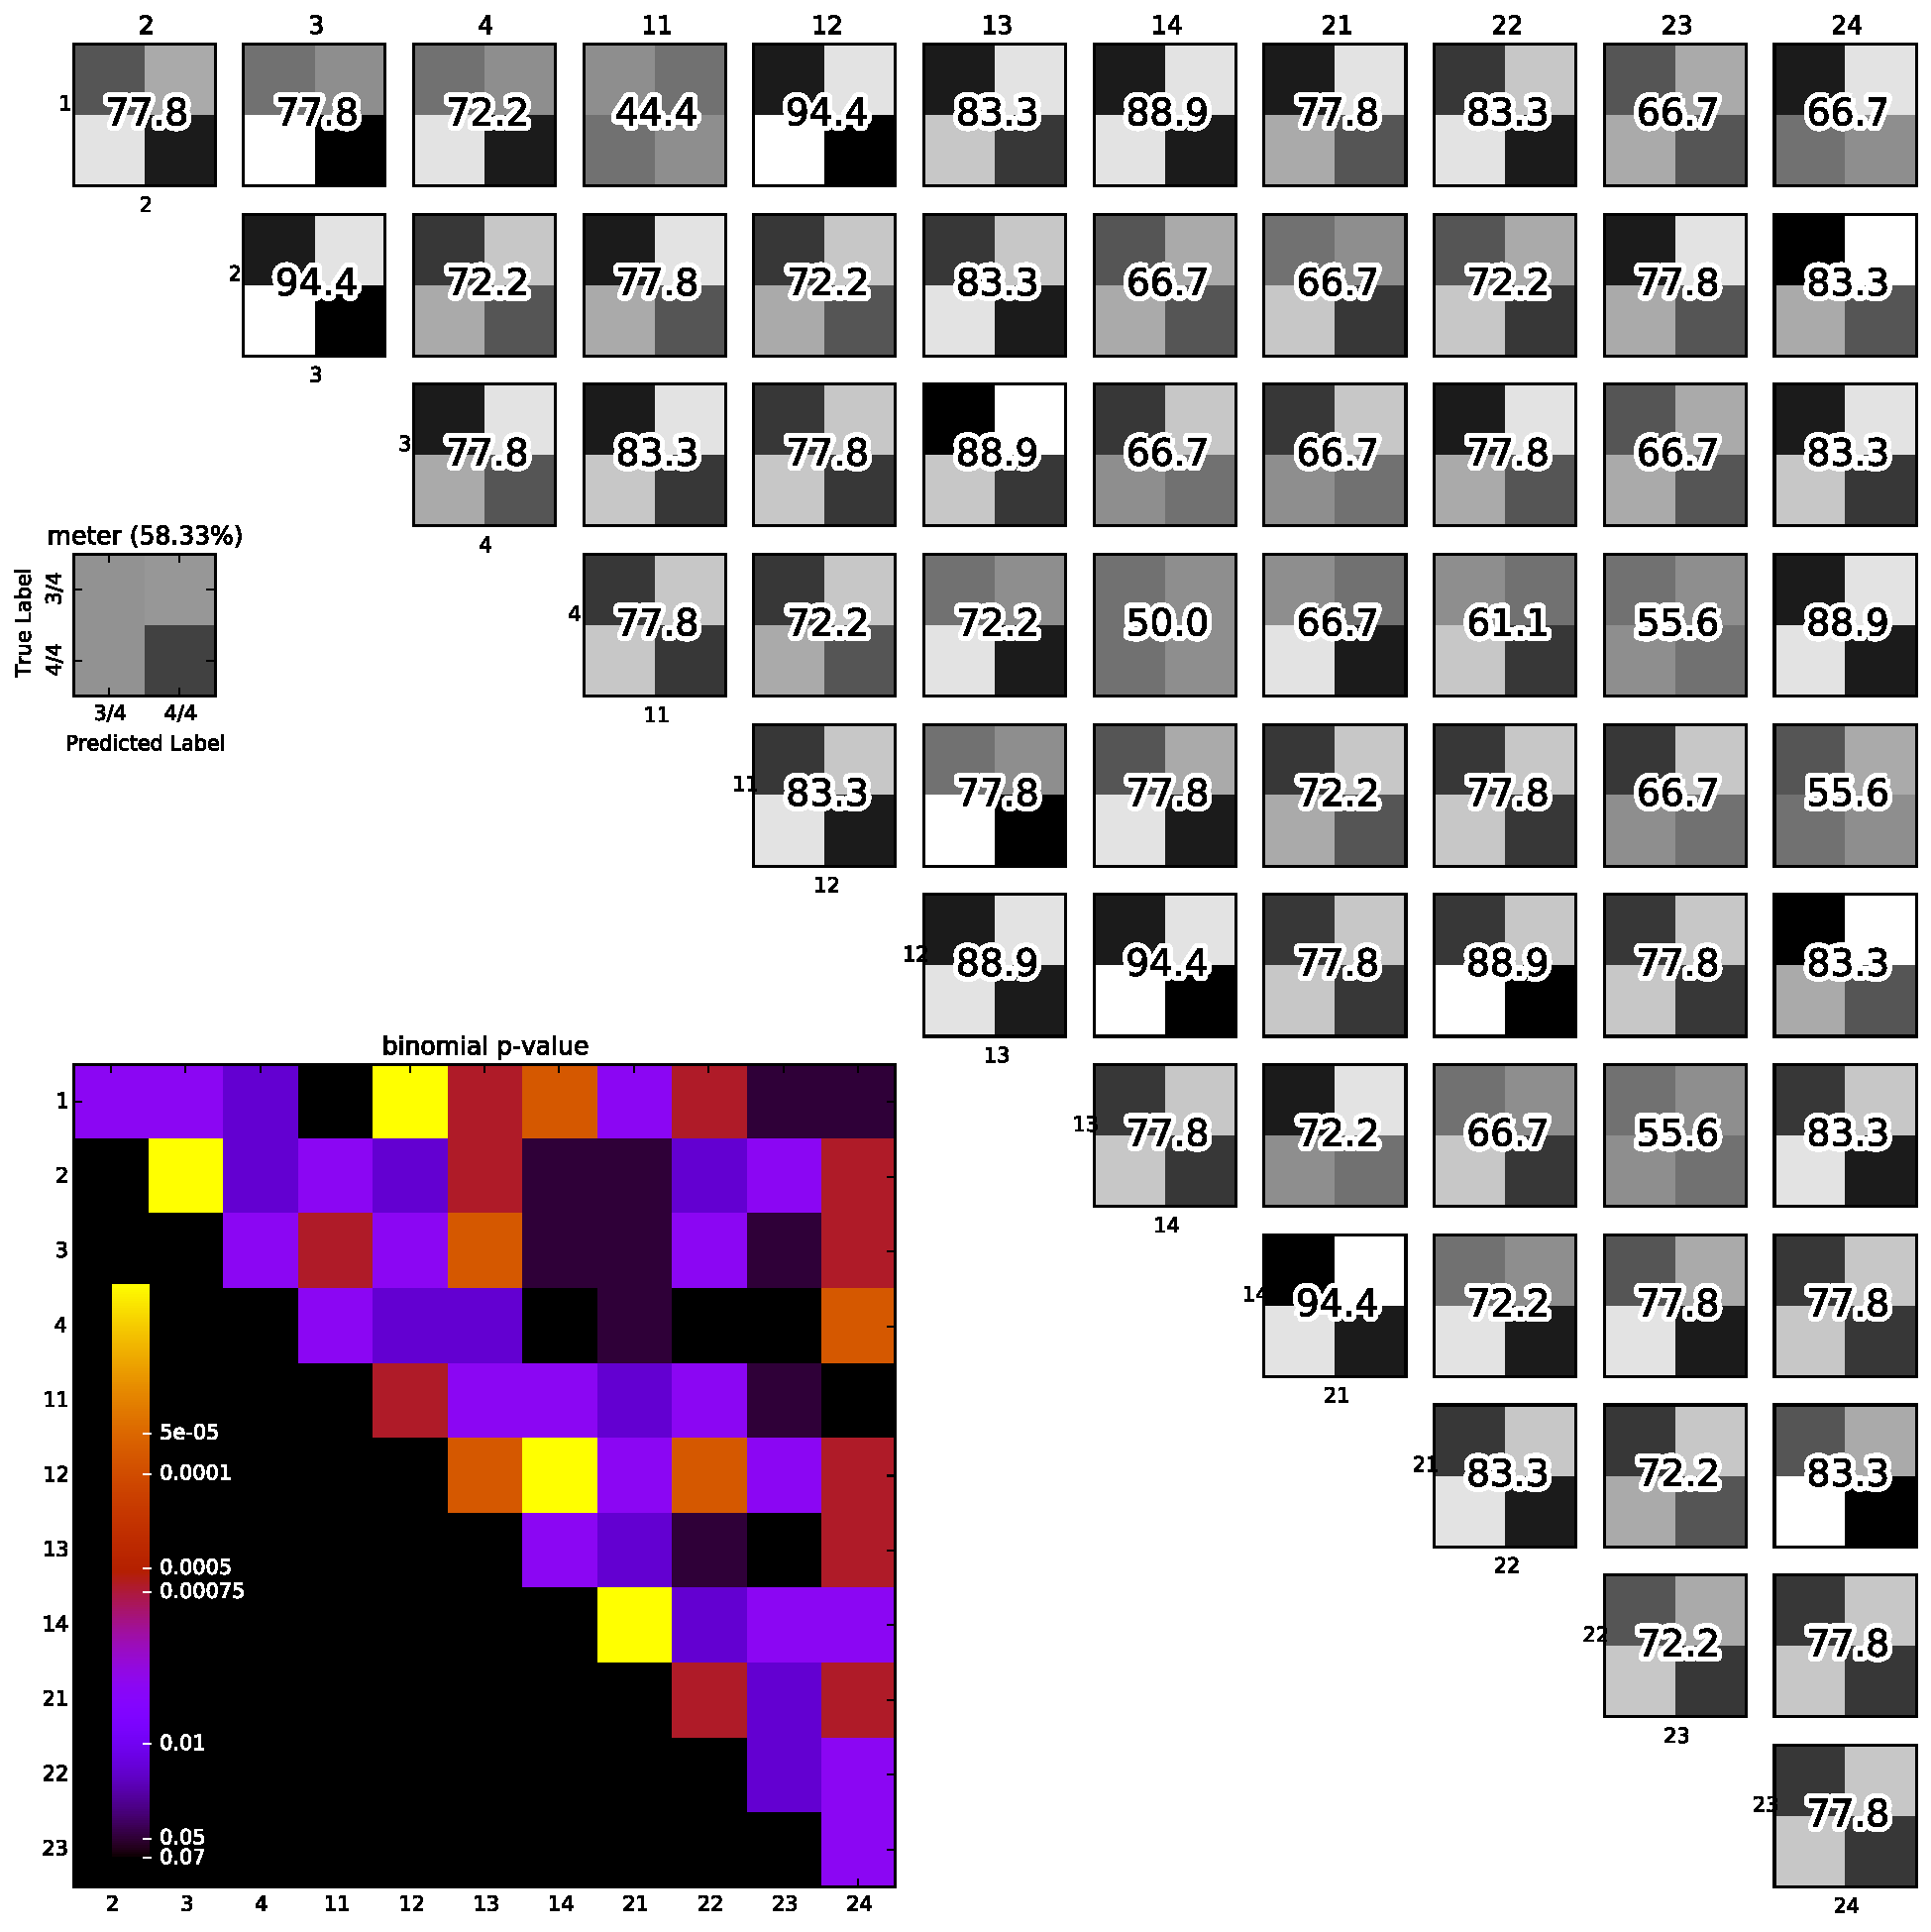
\includegraphics[width=.75\textwidth,keepaspectratio=true]{Figures/model_W_binary_confusion}
   \\\vspace{-0.8em}
    \caption{Binary confusion matrices for perception data.
    For each binary classification, only the 18 test trials belonging to either stimulus class A or stimulus class B were considered.
    The inset at the lower bottom visualizes the p-values determined by using the cumulative binomial distribution to estimate the likelihood of observing the respective binary classification rate by chance.}
    \label{fig:model_W_binary_confusion}
  \end{center}
  \vspace{-1em}
\end{figure}
For example: Chim Chim Cheree with lyrics is classified correctly 100\% of the time when paired with Jingle Bells without lyrics. 
Within each binary confusion matrix chance is 50\%.
The statistical significance (p-value)of each of the comparisons can be visualized in the figure's inset. 
Most of the binary comparisons are classified at a statistically significant level (p$<$0.05). 

The imagination data was then tested on the same model. 
The model was not able to classify the 12-classes. 
\autoref{fig:model_W_confusion_cond2} is a confusion matrix which shows the imagination classification results at 7.41\% (below chance). 
\begin{figure}[htb] 
  \begin{center}
    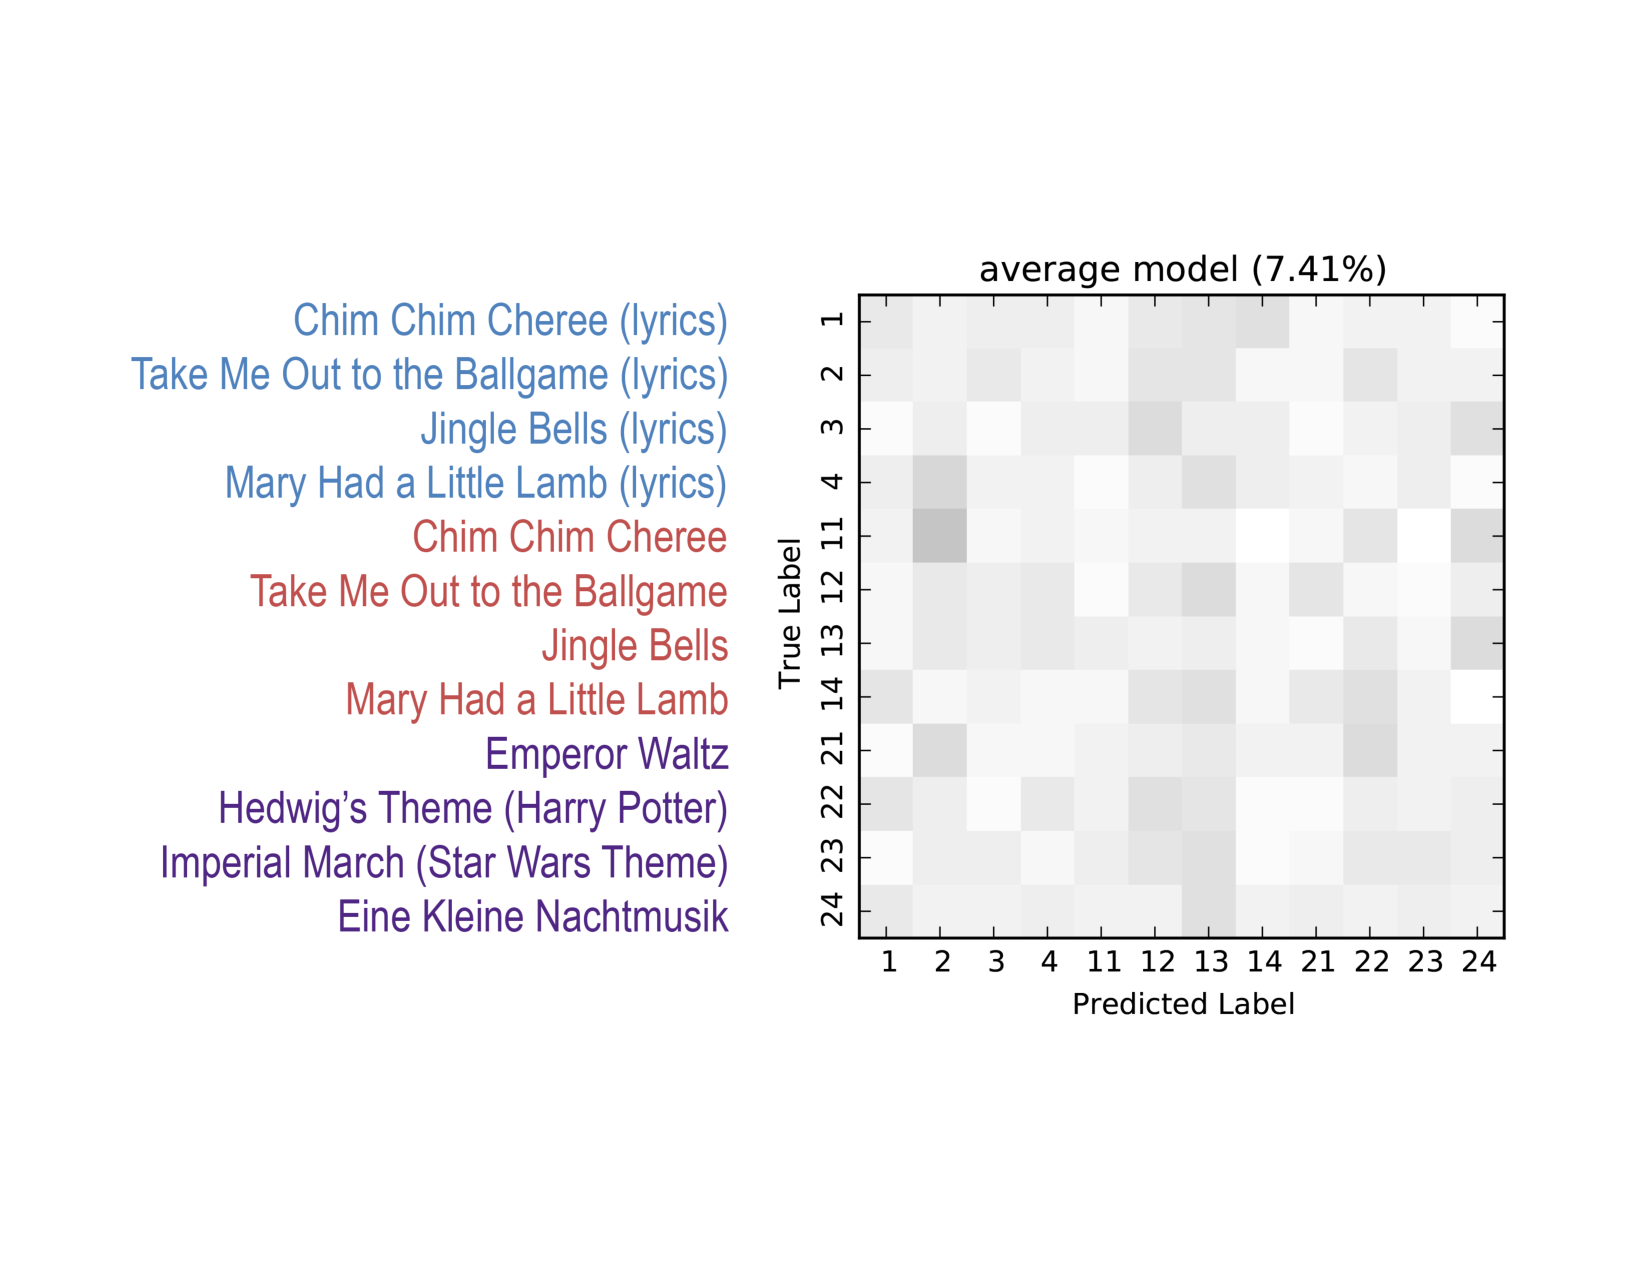
\includegraphics[width=.83\textwidth,keepaspectratio=true]{Figures/model_W_confusion_cond2}
   \\\vspace{-0.8em}
    \caption{12-class confusion matrix for imagination data. Colour indicates the number of times each selection was made with darker colours indicating more selections.}
        \label{fig:model_W_confusion_cond2}
  \end{center}
  \vspace{-1em}
\end{figure}

We investigated whether there were pairs of imagined stimuli that the model could accurately classify. 
\autoref{fig:model_W_binary_confusion_cond2} shows the binary confusion matrix.
Most of the stimuli pairs are not classified at a statistically significant level. 
However, there is one binary comparison that stands out. 
Stimulus 1 with 12 is classified at a rate of 62.2\% (p$<$0.05). 
It is interesting to note that this does not mirror what is seen in the binary comparisons of perception data, where the most classifiable pair was stimulus 1 with 13. 
\begin{figure}[h] 
  \begin{center}
    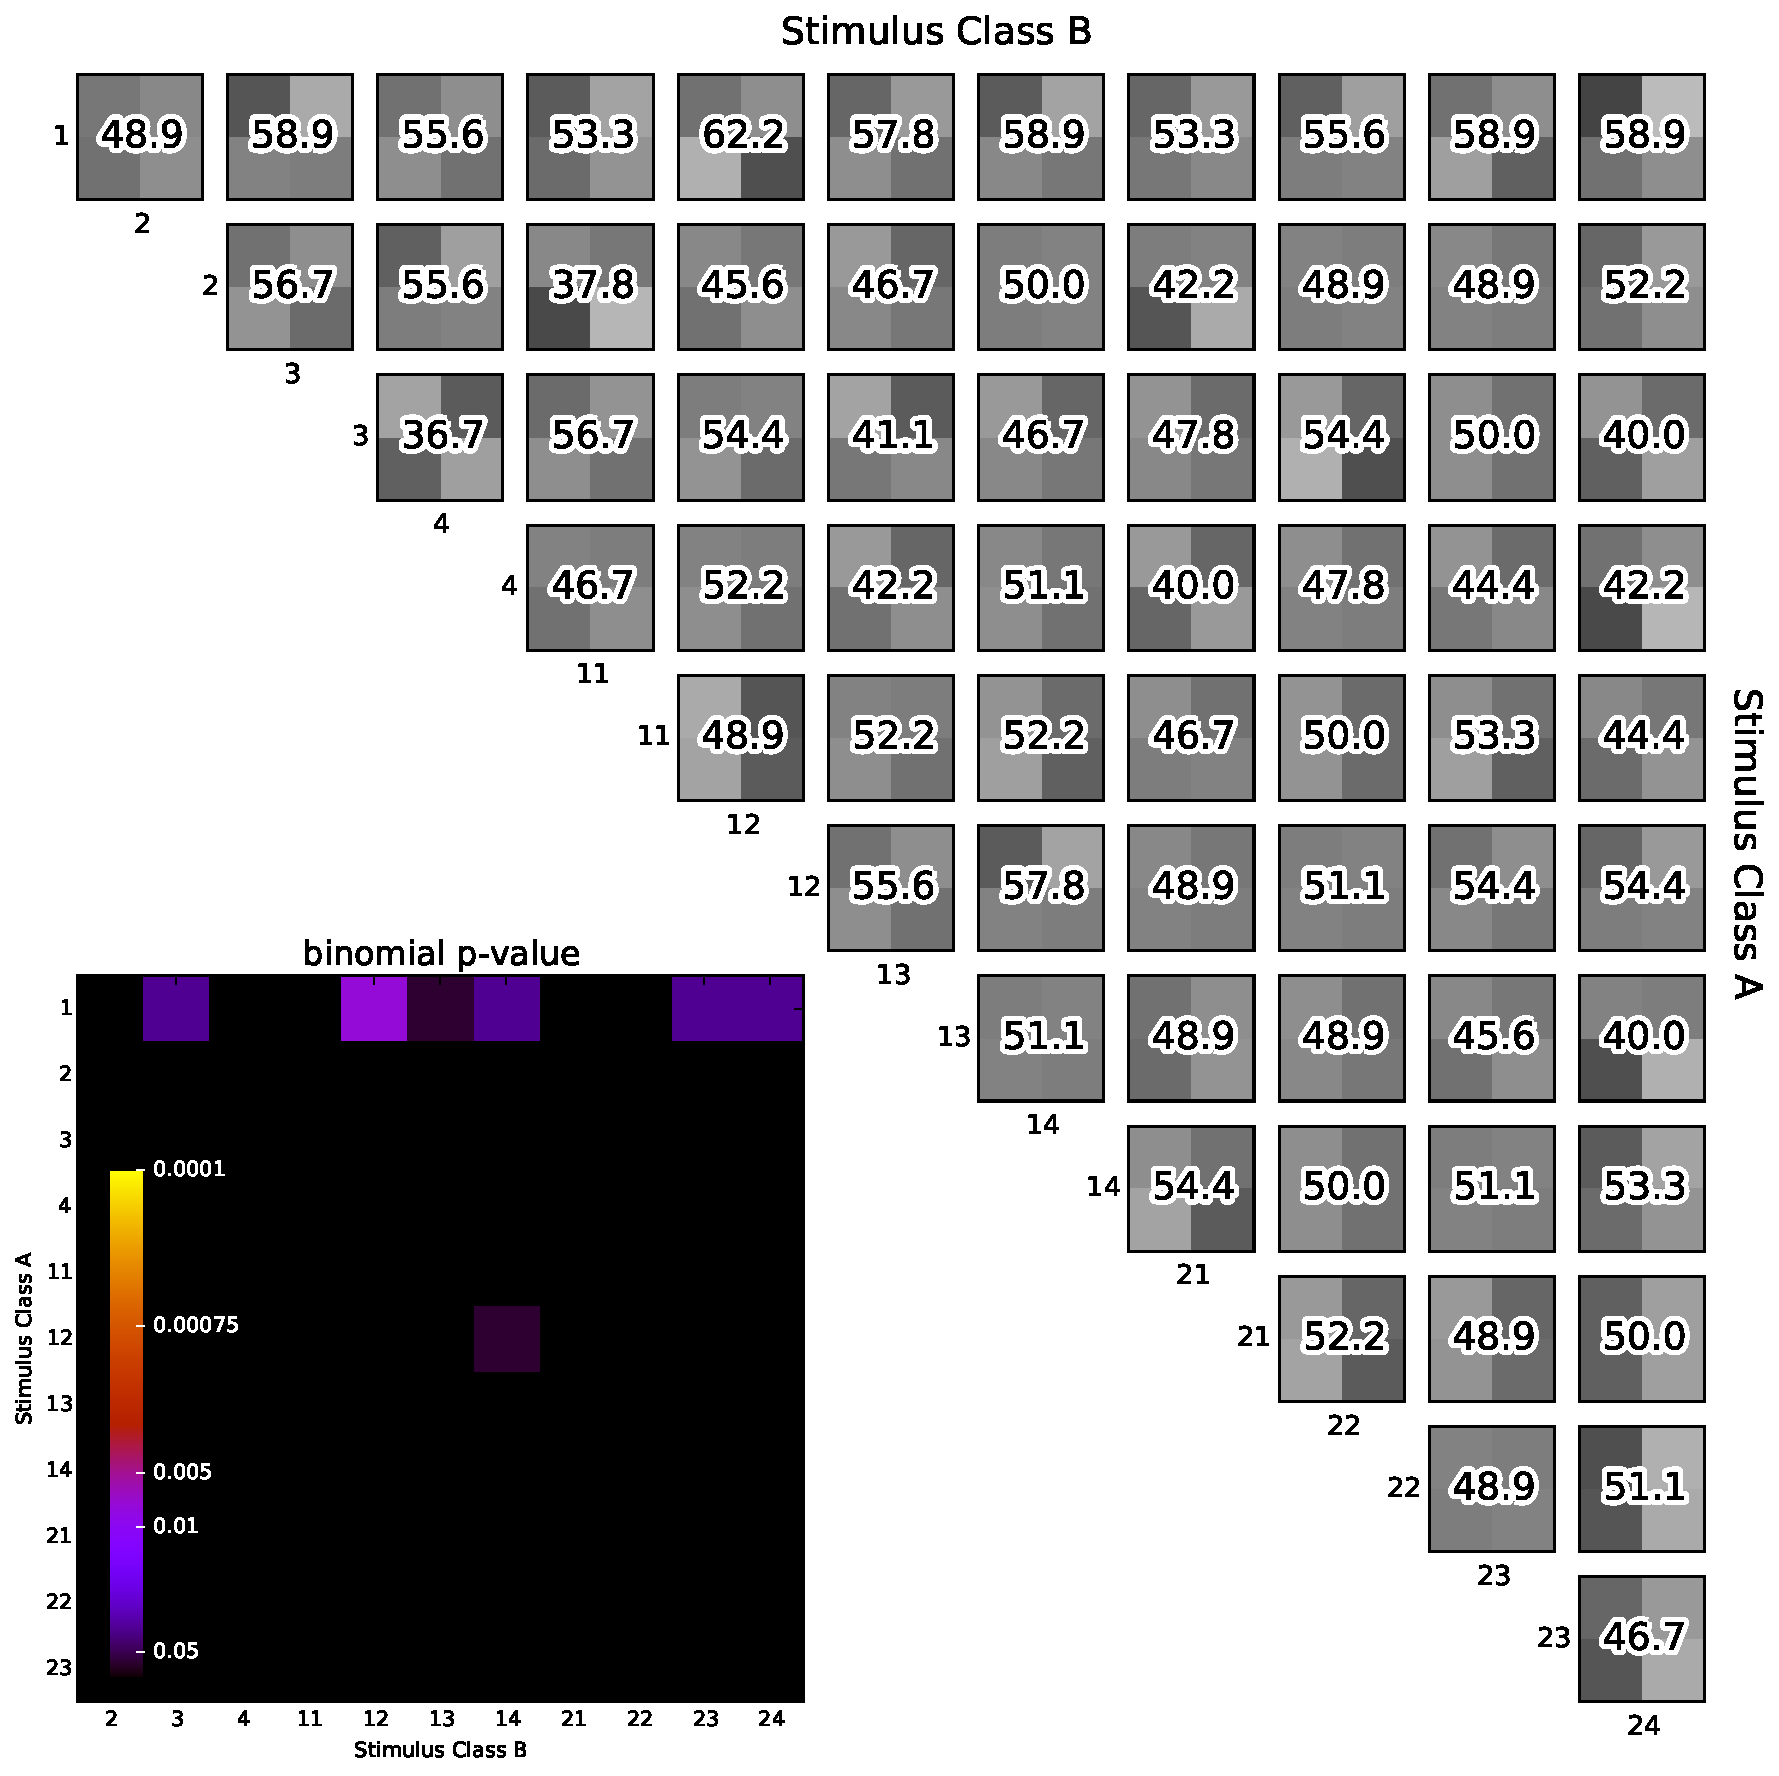
\includegraphics[width=.75\textwidth,keepaspectratio=true]{Figures/model_W_binary_confusion_cond2}
   \\\vspace{-0.8em}
    \caption{Binary confusion matrices for imagination data.
    For each binary classification, only the 18 test trials belonging to either stimulus class A or stimulus class B were considered.
    The inset at the lower bottom visualizes the p-values determined by using the cumulative binomial distribution to estimate the likelihood of observing the respective binary classification rate by chance.}
    \label{fig:model_W_binary_confusion_cond2}
  \end{center}
  \vspace{-1em}
\end{figure}
\newpage
\section{Discussion}
The neural net does not give us information about what characteristics it is using to classify the stimuli, and it is difficult to interpret from the results what signals the brain is producing that allow this classification to occur. 
In layer three of \autoref{fig:model_W} we see compressed representations of the EEG data for each stimuli. 
One characteristic of these representations are the dark red bands that stand out from the rest of the time course. 
These red bands indicate time periods that the neural net has identified as being important for classification. 
When taking a closer look we see that these bands line up for lyric/non-lyric pairs of stimuli. 
For example the darkest red band in stimulus 1 appears at a very similar time point as the darkest red band in stimulus 11.
A similar pattern can be seen in stimuli 2/12 and 3/13.
Upon investigation of the audio of the stimuli there were no characteristics that stood out as driving these important time periods.
It is possible that these red bands represent a cognitive process, such as recognition, that occurs at these time points during perception of the stimuli. 
To investigate this possibility we ran a follow-up behavioural experiment asking participants to indicate when they consciously recognized each stimulus. 
This experiment is described in the next section.

The results of our neural net show that some stimuli are better classified than others, and some pairs of stimuli are more easily differentiated. 
To investigate whether the neural net is using a comparison system similar to what humans might employ we decided to run a follow-up, behavioural experiment asking participants to rate the similarity of pairs of stimuli. 

